\chapter{How to prove it?}
\begin{figure}[htp]
	\centering
	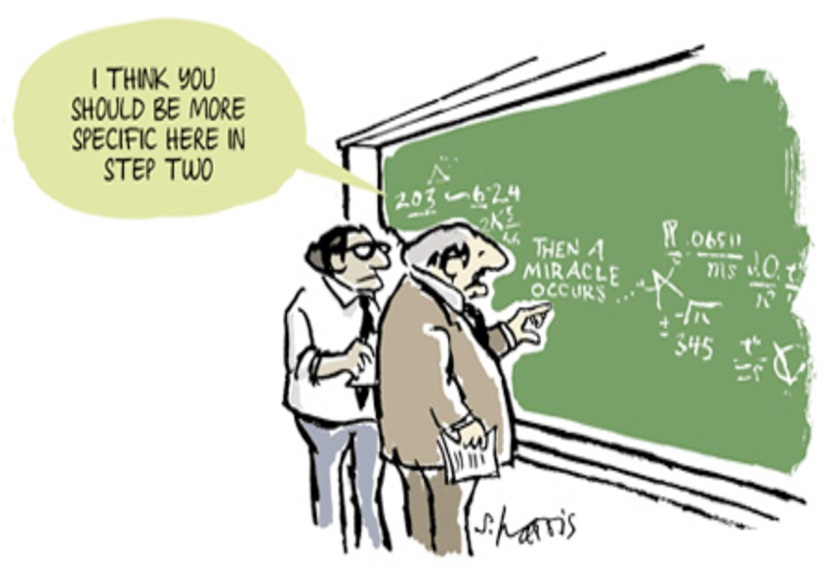
\includegraphics[width=\linewidth]{Assets/0_W-tEtGVYH9eM9HNx}
	\caption{}
	\label{fig:specific}
\end{figure}

One of the largest stumbling block in studying mathematics is learning how to prove theorems. In this post, I would share with you 3 of the most commonly used technique with at least one step by step example.
\newpage
\noindent \textbf{1. Direct proof}

\noindent Perhaps the most intuitive and straightforward way to write proofs. It goes by "\textit{If A, then B}" or  "\textit{A implies B}" or mathematically A $\Rightarrow$ B.

\noindent\textbf{Example 1} : \textit{The sum of two even numbers is also even.}
\begin{proof}
	Let \textit{x} and \textit{y} be even numbers. Since they are even, by definition they can be rewritten as \textit{2n} and \textit{2m} respectively. Thus, the sum \textit{x+y = 2n+2m = 2(n+m)}, which is even number by definition.
\end{proof}
\noindent\textbf{Example 2} : \textit{Third Binomial Formula}
\begin{proof}
\begin{align}
(a-b)\cdot (a+b)&= a\cdot a+a\cdot b-b \cdot a-b \cdot b\\ 
			&= a^2+a \cdot b-b \cdot a-b^2\\ 
			&= a^2-b^2 
\end{align}
\end{proof}
\noindent\textbf{Example 3} : \textit{Square of odd number is also odd}

\noindent \textbf{2. Indirect proof or proof by contradiction}

\noindent\textbf{Example 4} : \textit{Square root of two is irrational}

